\documentclass{article}
\usepackage[T1]{fontenc}
\usepackage{lmodern}
\usepackage{graphicx}
\usepackage{amsmath,amssymb}
\usepackage[a4paper,margin=2cm]{geometry}
\usepackage[absolute,overlay]{textpos}
\setlength{\TPHorizModule}{1mm}
\setlength{\TPVertModule}{1mm}
\usepackage[indonesian]{babel}
\usepackage{hyperref}
\setlength{\emergencystretch}{2em}
% unit: Halaman 38

\begin{document}

% === Halaman 38 (llm) ===

# Program utamaPembangkitanKunciRSA()

\vspace{86.13mm}

\begin{verbatim}
pesan = input("Ketikkan pesan teks: ")
ciphertext = encrypt_message(pesan, 'kunci_publik.pem')
print("\nCiphertext:", ciphertext.hex())

decrypted_message = decrypt_message(ciphertext, 'kunci_privat.pem')
print("\nPesan setelah dekripsi:", decrypted_message)
\end{verbatim}

% deskripsi: Potongan kode program Python untuk proses enkripsi dan dekripsi menggunakan algoritma RSA.
% bbox normalisasi: [0.0800, 0.1800, 0.8400, 0.4700]
\begin{textblock*}{159.60mm}(16.80mm,53.46mm)
\noindent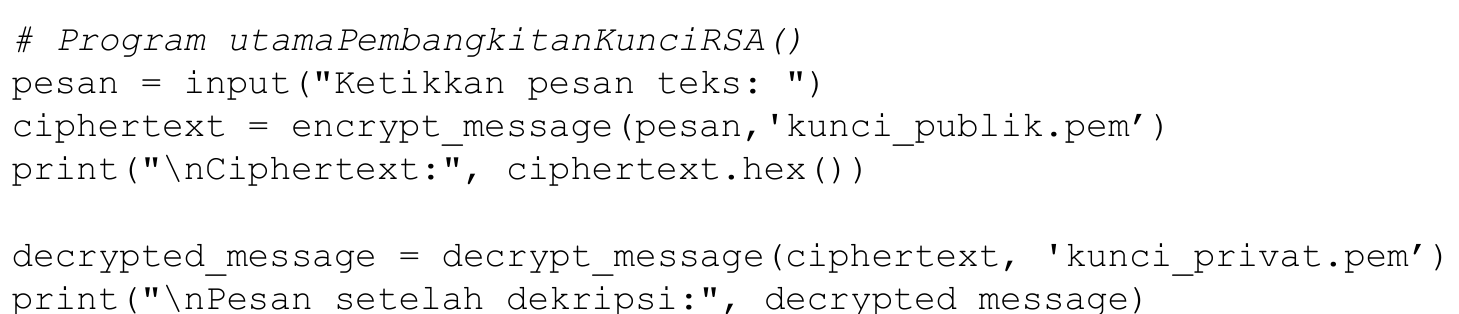
\includegraphics[width=159.60mm,height=86.13mm]{../../images/llm/page_038_img_01.png}%
\end{textblock*}

\end{document}
